\chapter{\uppercase{Neutrino Oscillation in the PROSPECT AD}}

\section{Detecting Antineutrinos}

PROSPECT detects $\bar{\nu_e}$'s via the inverse beta decay reaction (IBD):
\begin{equation}
	\bar{\nu_e} + p \rightarrow e^+ + n
\end{equation}
A reactor $\bar{\nu_e}$ will interact with a proton in the $^6$Li-LS, producing a positron and a neutron.
The positron will quickly lose energy and annihilate with an electron, producing two 511 keV $\gamma$-rays.
This is the prompt signal.

Concurrently, the neutron will thermalize by scattering off of protons in the scintillator until it captures on $^6$Li ($\sim$80\% of the time) or H ($\sim$20\% of the time).
The neutron capture on $^6$Li (nLi) produces a tritium and an alpha with energies 2.05 MeV and 2.75 MeV respectively. 
These two products will immediately scintillate, and produce a quenched signal of $\sim$0.55 MeVee.
This is the delayed signal.
Figure~\ref{fig:ibd} illustrates this process in the PROSPECT LiLS.

The neutron capture on $^6$Li takes $\sim$40$\mu$s, providing a time separation between the prompt and delayed signals.
Making use of the time coincident, PSD, and energy cuts, PROSPECT can identify $\bar{\nu_e}$ events above background. 

\begin{figure}[!t]
	\centering
	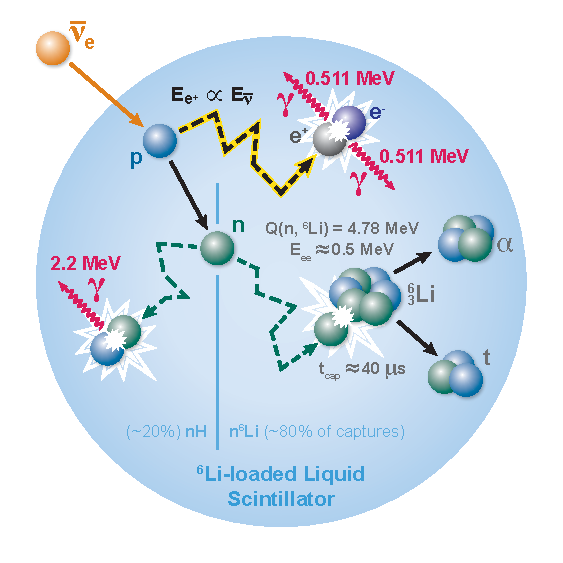
\includegraphics[width=0.4\linewidth]{tex/7-oscillation-images/IBD}
	\caption{Schematic of the IBD interaction is the PROSPECT AD.}
	\label{fig:ibd}
\end{figure}

\section{IBD Event Selection}

\subsection{Cuts}

A selection of energy, PSD, and time cuts, along with specified event vetos are utilized to identify IBD signals and reduce background.
These are:
\begin{itemize}
	\item Prompt Cluster Size: $\geq1$
	\item Prompt PSD: All pulses must have PSD that is $<3\sigma$ from the gamma-like PSD band mean
	\item Prompt Energy: No cut, but only clusters with a total energy of 0.8 $<$ E$_{\textrm{rec}} <$ 7.2 MeV are used in the oscillation analysis
	\item Delayed Cluster Size: Single pulse
	\item Delayed PSD: All pulses must have PSD that is $>3.6\sigma$ from the gamma-like PSD band mean
	\item Delayed Energy: 0.46 $<$ E$_{\textrm{rec}} < $0.60 MeV
	\item Time Correlation: $\Delta t = (1,120)~\mu$s
	\item Prompt-Delayed Distance: $\Delta z <$ 18 cm for coincidences in the same segment; $\Delta z <$ 14 cm for coincidences in horizontally/vertically adjacent segments
	\item Pileup Veto: Applied to both prompt and delayed clusters, if the candidate cluster is preceded by another cluster in a window of $<$ 800 ns, the candidate cluster is vetoed
	\item Shower Veto: Veto delayed clusters that exist in a (0,100) $\mu$s window around cosmic muon clusters (E$_{\textrm{rec}} >$ 15 MeV); Veto delayed clusters that exist within (-200,+200)~$\mu$s of events with PSD $> 3\sigma$ from the gamma-like PSD band mean and E $>$ 0.25 MeV
	\item Fiducialization: Reject events in which a prompt or delayed event occurs in the outer ring of segments; reject events that occur outside of $z$ = (-448, 448) mm 
\end{itemize}
For an example of how the PSD and energy cuts look in PSD versus energy space for prompt events correlated with a delayed neutron capture see Figure~\ref{fig:psdvsecorrnli}.

\begin{figure}[h]
	\centering
	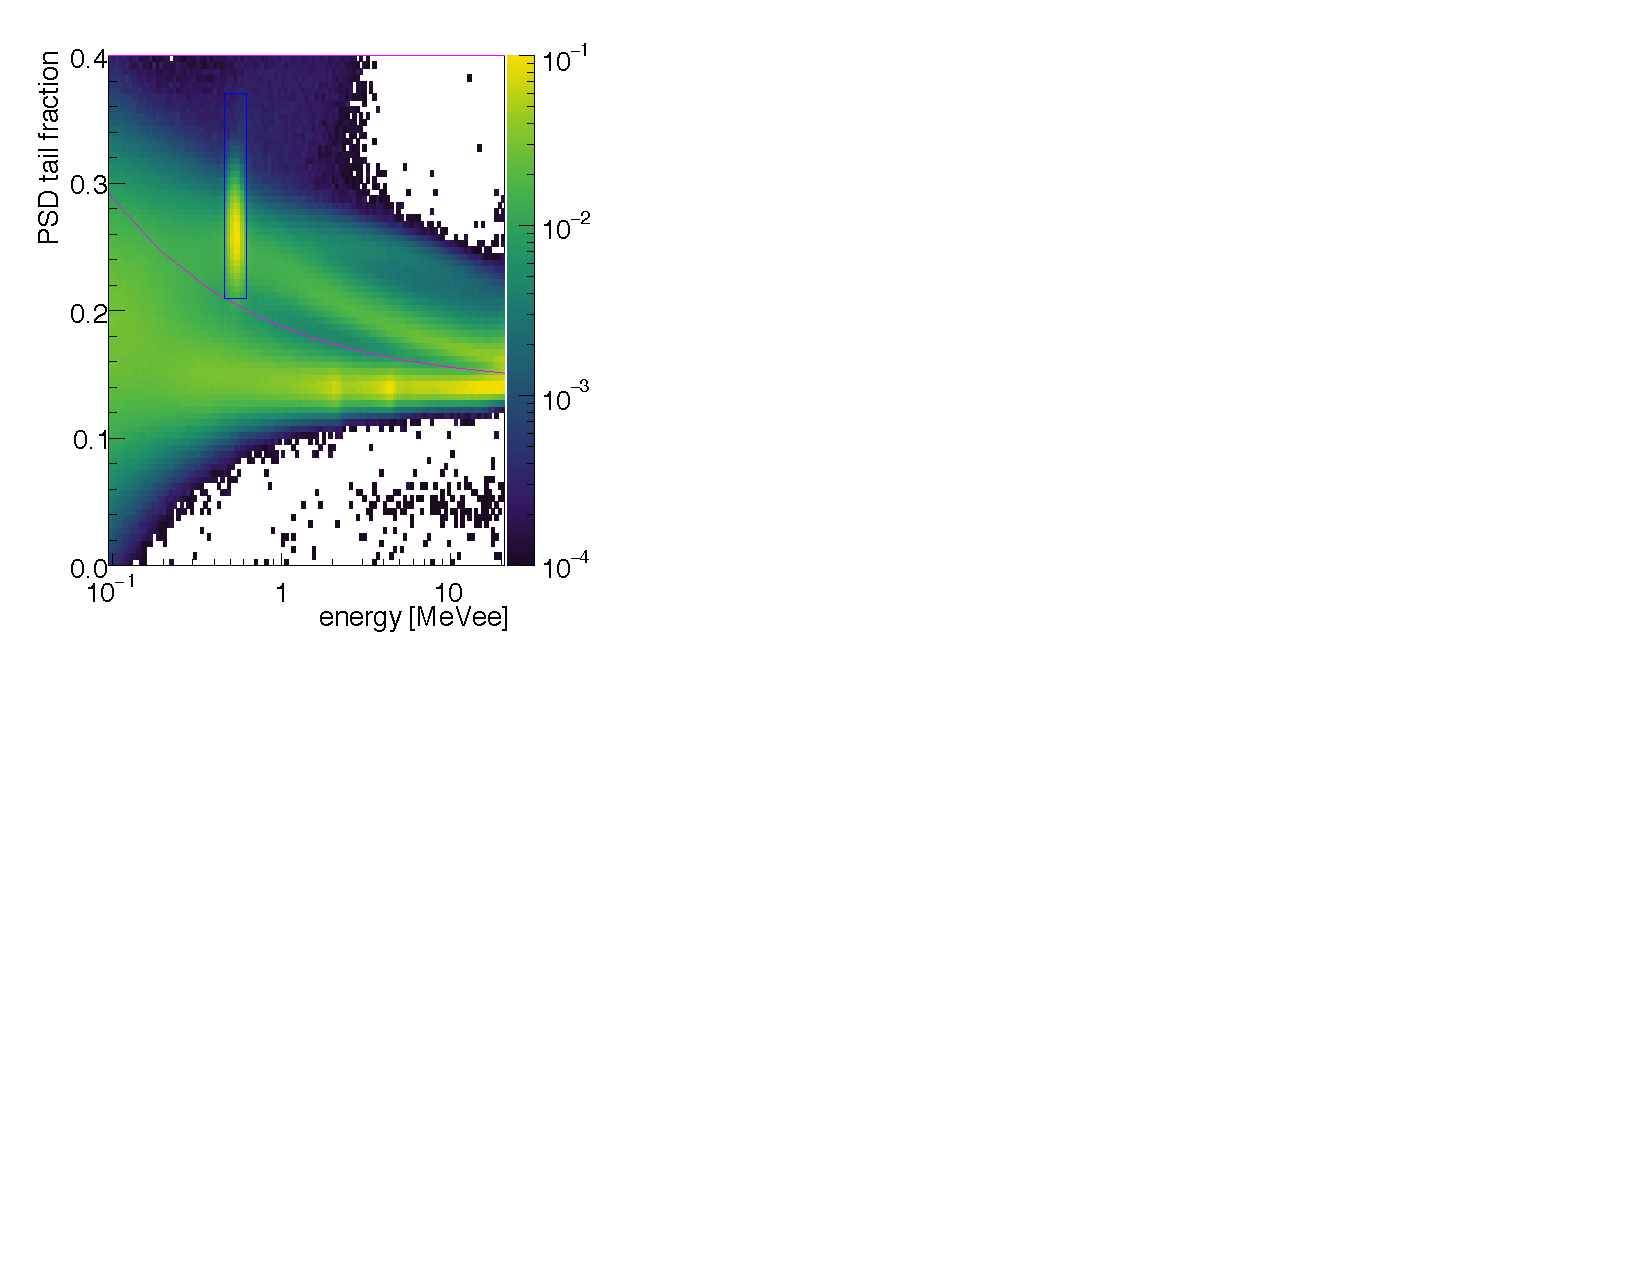
\includegraphics[width=0.6\linewidth]{tex/7-oscillation-images/PSDvsE_Corr_nLi}
	\caption{PSD versus energy distribution for prompt events correlated with a delayed neutron capture on $^6$Li. The cuts used for identifying nLi events is represented by the blue rectangle. The upper limit of the cut used for identifying electron-like signals is shown as the pink curve.}
	\label{fig:psdvsecorrnli}
\end{figure}



\subsection{Backgrounds}

The two primary backgrounds to the IBD signal are time-correlated cosmogenic neutron events and accidental coincidences of ambient $\gamma$-rays and nLi captures.
Cosmic muons moving through the lead shielding can create multiple neutrons that may be selected as delayed events.
The shower veto helps to reduce this background, introducing a dead-time that varies between 5.5\% and 6.9\% for reactor off and on times respectively.
Along with this veto, the IBD selection is applied to reactor off data and the resulting distributions are subtracted from the reactor on results.

Accidental coincidences are handled by selecting prompt-delay pairs with $\Delta t$ = (-12,-2) ms.
This provides a high statistics sample of events that are scaled to match the correlated time window and then subtracted from the correlated events. 
This is done for both reactor on and off data sets.

\begin{figure}[!b]
	\centering
	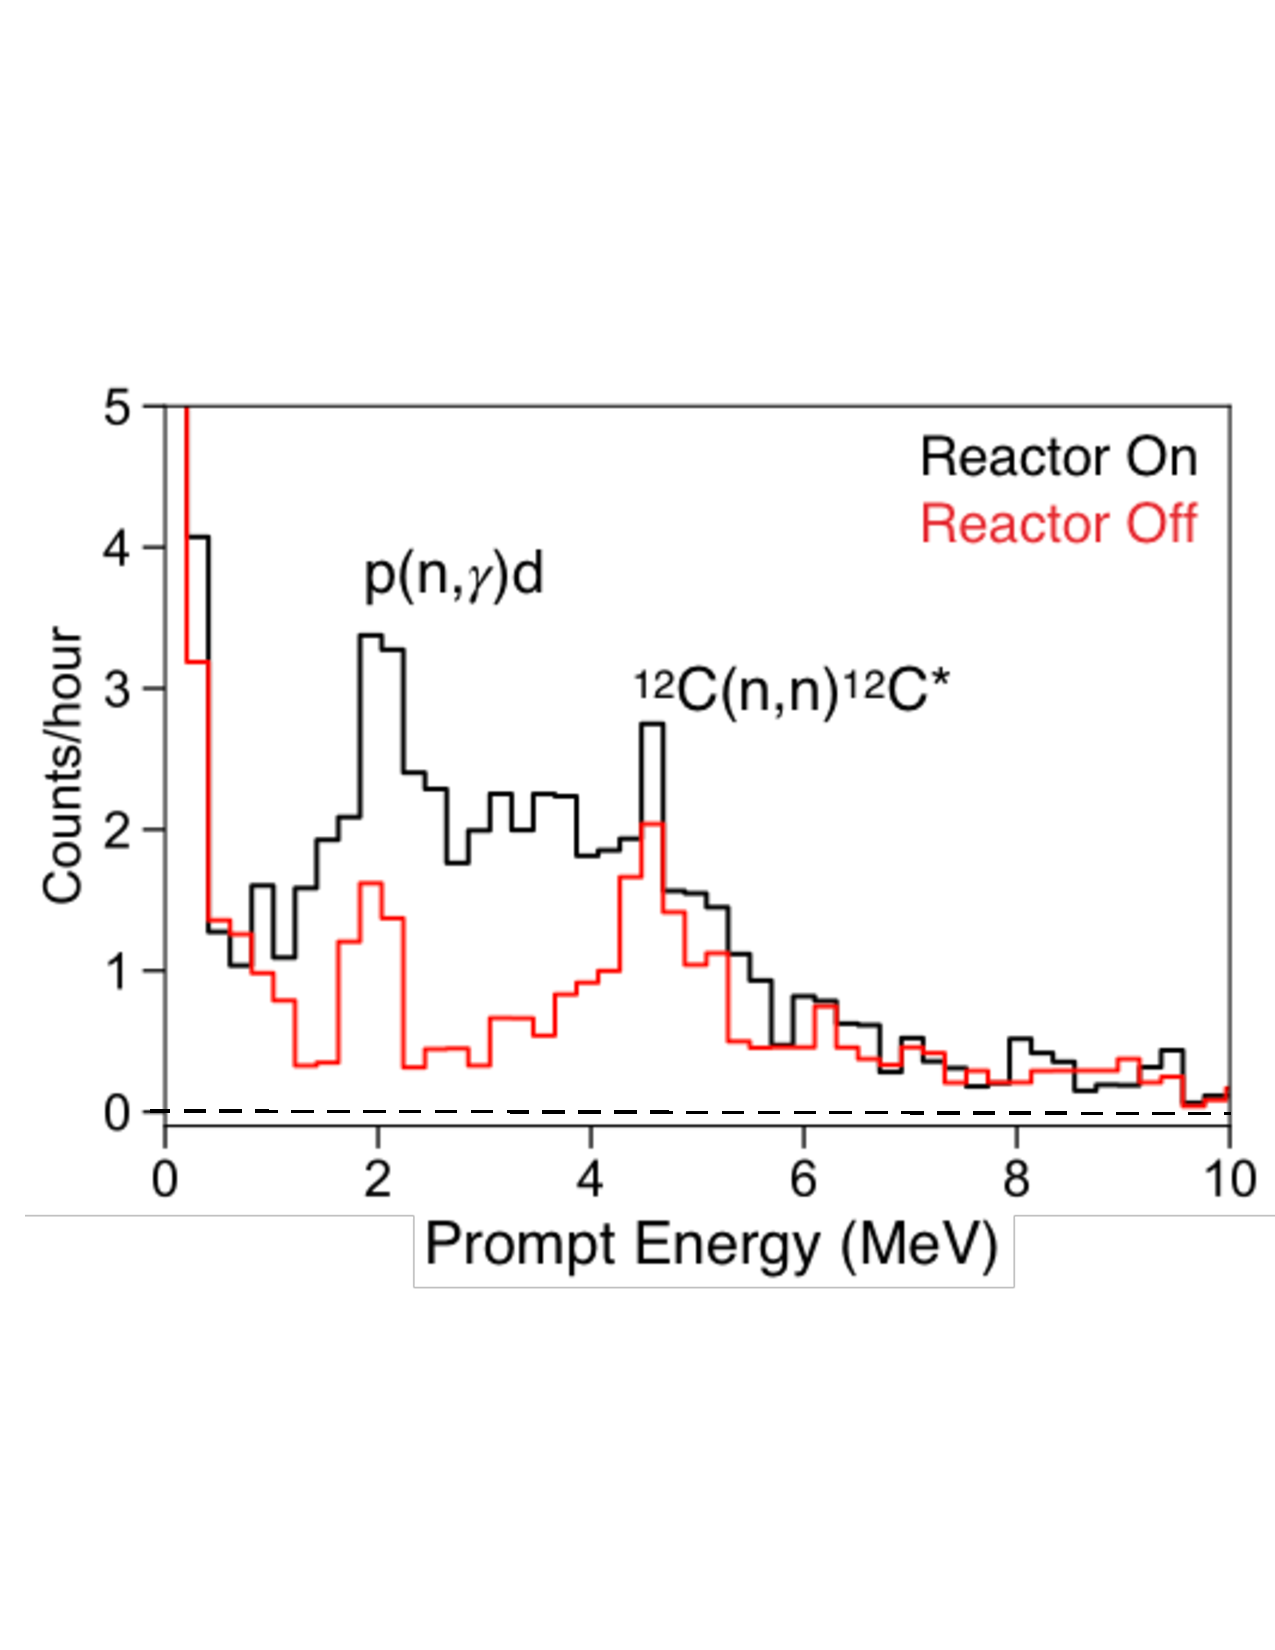
\includegraphics[width=0.6\linewidth]{tex/7-oscillation-images/IBD_E}
	\caption{The prompt energy spectra, after background subtraction, of IBD events for 24 hours of both reactor on and off data. Prominent peaks at 2.2 MeV and 4.4 MeV are due to neutron captures on Hydrogen and inelastic neutron scatters on $^{12}$C respectively.}
	\label{fig:ibde}
\end{figure}

Figure~\ref{fig:ibde} shows the prompt energy spectra for 24 hours both of reactor on and off data after applying all cuts and accidental background subtraction.
Prominent peaks at 2.2 MeV and 4.4 MeV exist in both reactor on and off data.
Cosmogenic muons can create several neutrons. One of these will capture on hydrogen (nH), producing a 2.2 MeV $\gamma$, which will be followed by another neutron capturing on $^6$Li. 
These time-coincident events are reduced by the shower veto, but not completely removed.

High energy neutrons (fast neutrons) will also inelastically scatter off of $^{12}$C in the scintillator causing the reaction:
\begin{equation}
	n + ^{12}C \rightarrow n' + ^{12}C^*
\end{equation}
As $^{12}$C$^*$ de-excites it will release a 4.4 MeV photon, while the scattered neutron thermalizes and captures on $^{6}$Li, mimicking the IBD signal.


\subsection{Atmospheric Correction}

Cosmogenic rates vary according to changes in pressure, therefore, a scaling factor for this effect needs to be introduced in order to perform accurate background subtraction.
To determine the size of this correction fast neutron events with a prompt proton recoil and a delayed nLi capture (FN+nLi) were studied. 
The prompt event was required to have PSD $>3\sigma$ from the gamma-like PSD band mean, otherwise all other cuts used were the same as the ones used for IBD selection.

\begin{figure}[!b]
	\begin{subfigure}{0.5\linewidth}
		\centering
		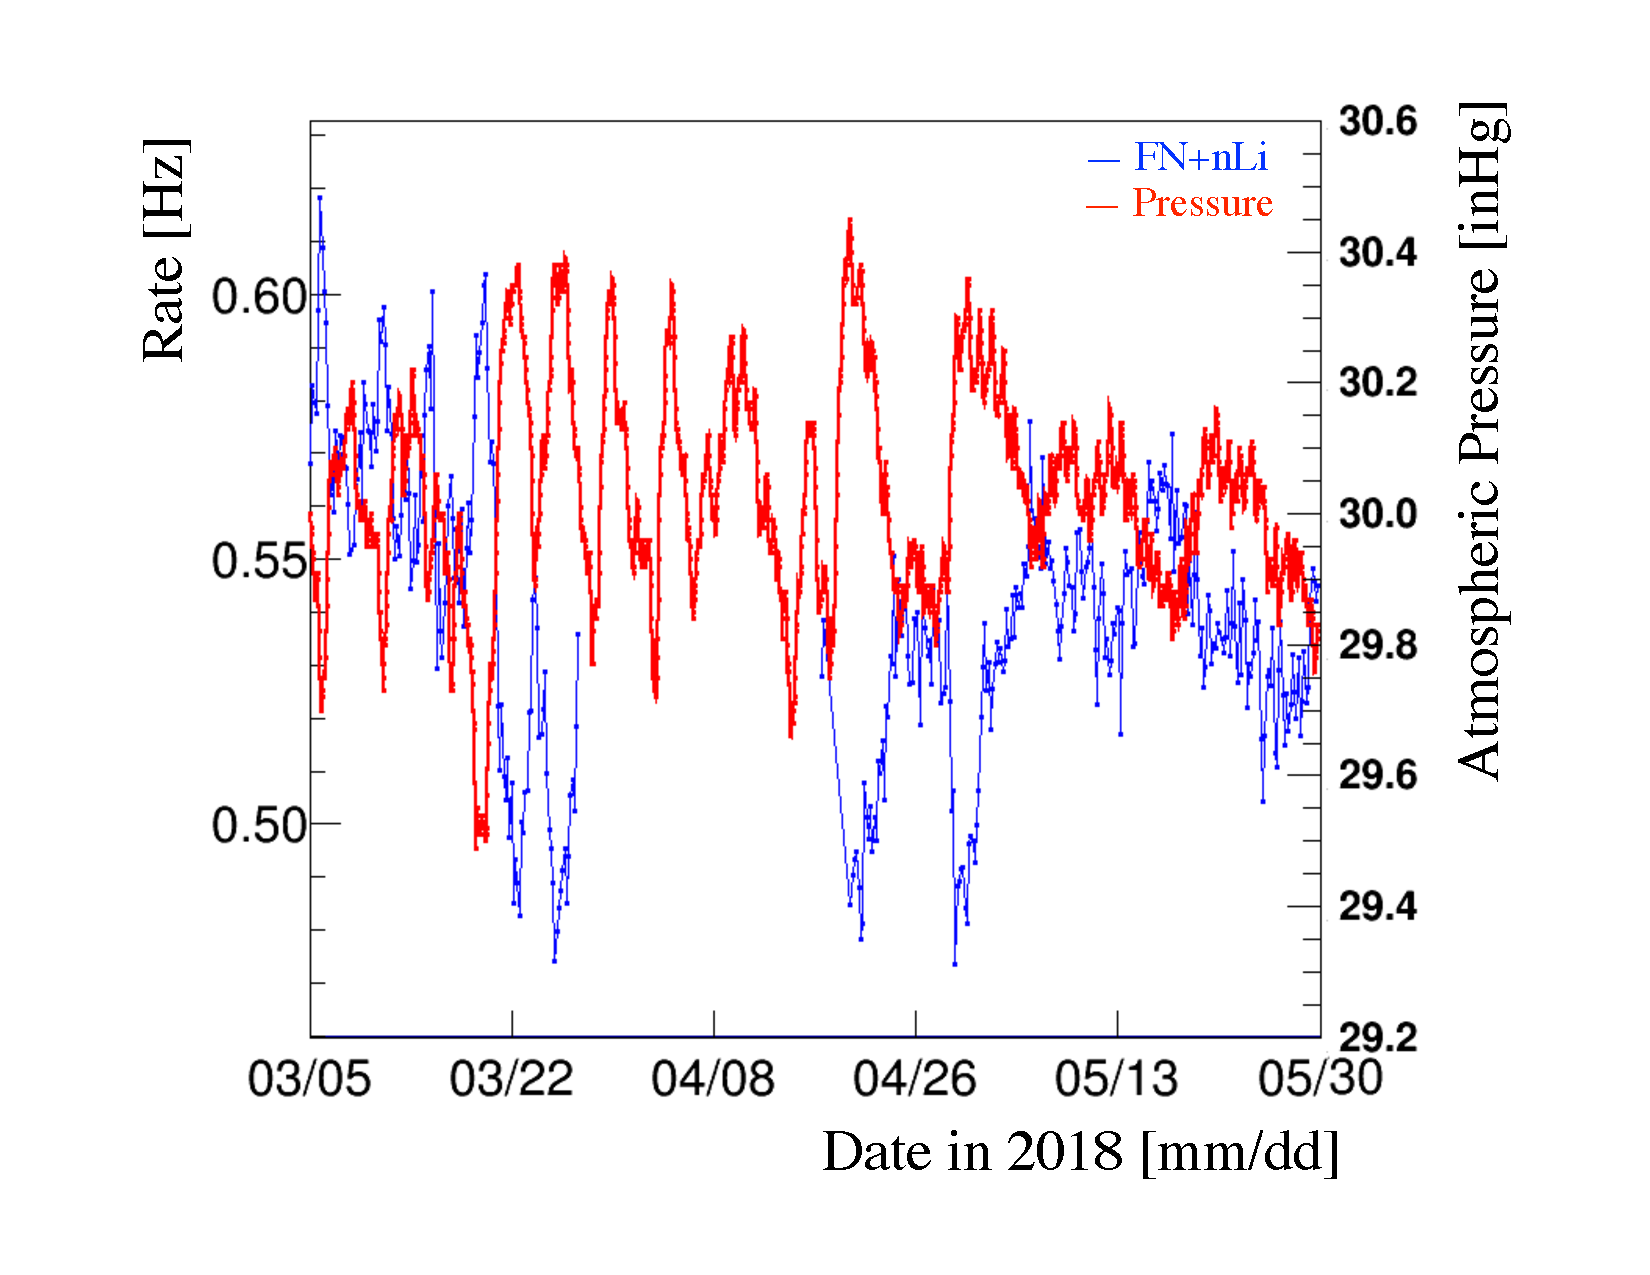
\includegraphics[width=0.95\linewidth]{tex/7-oscillation-images/FNnLi_Rate}
		%\caption{}
		\label{fig:fnnlirate}
	\end{subfigure}
	\begin{subfigure}{0.5\linewidth}
		\centering
		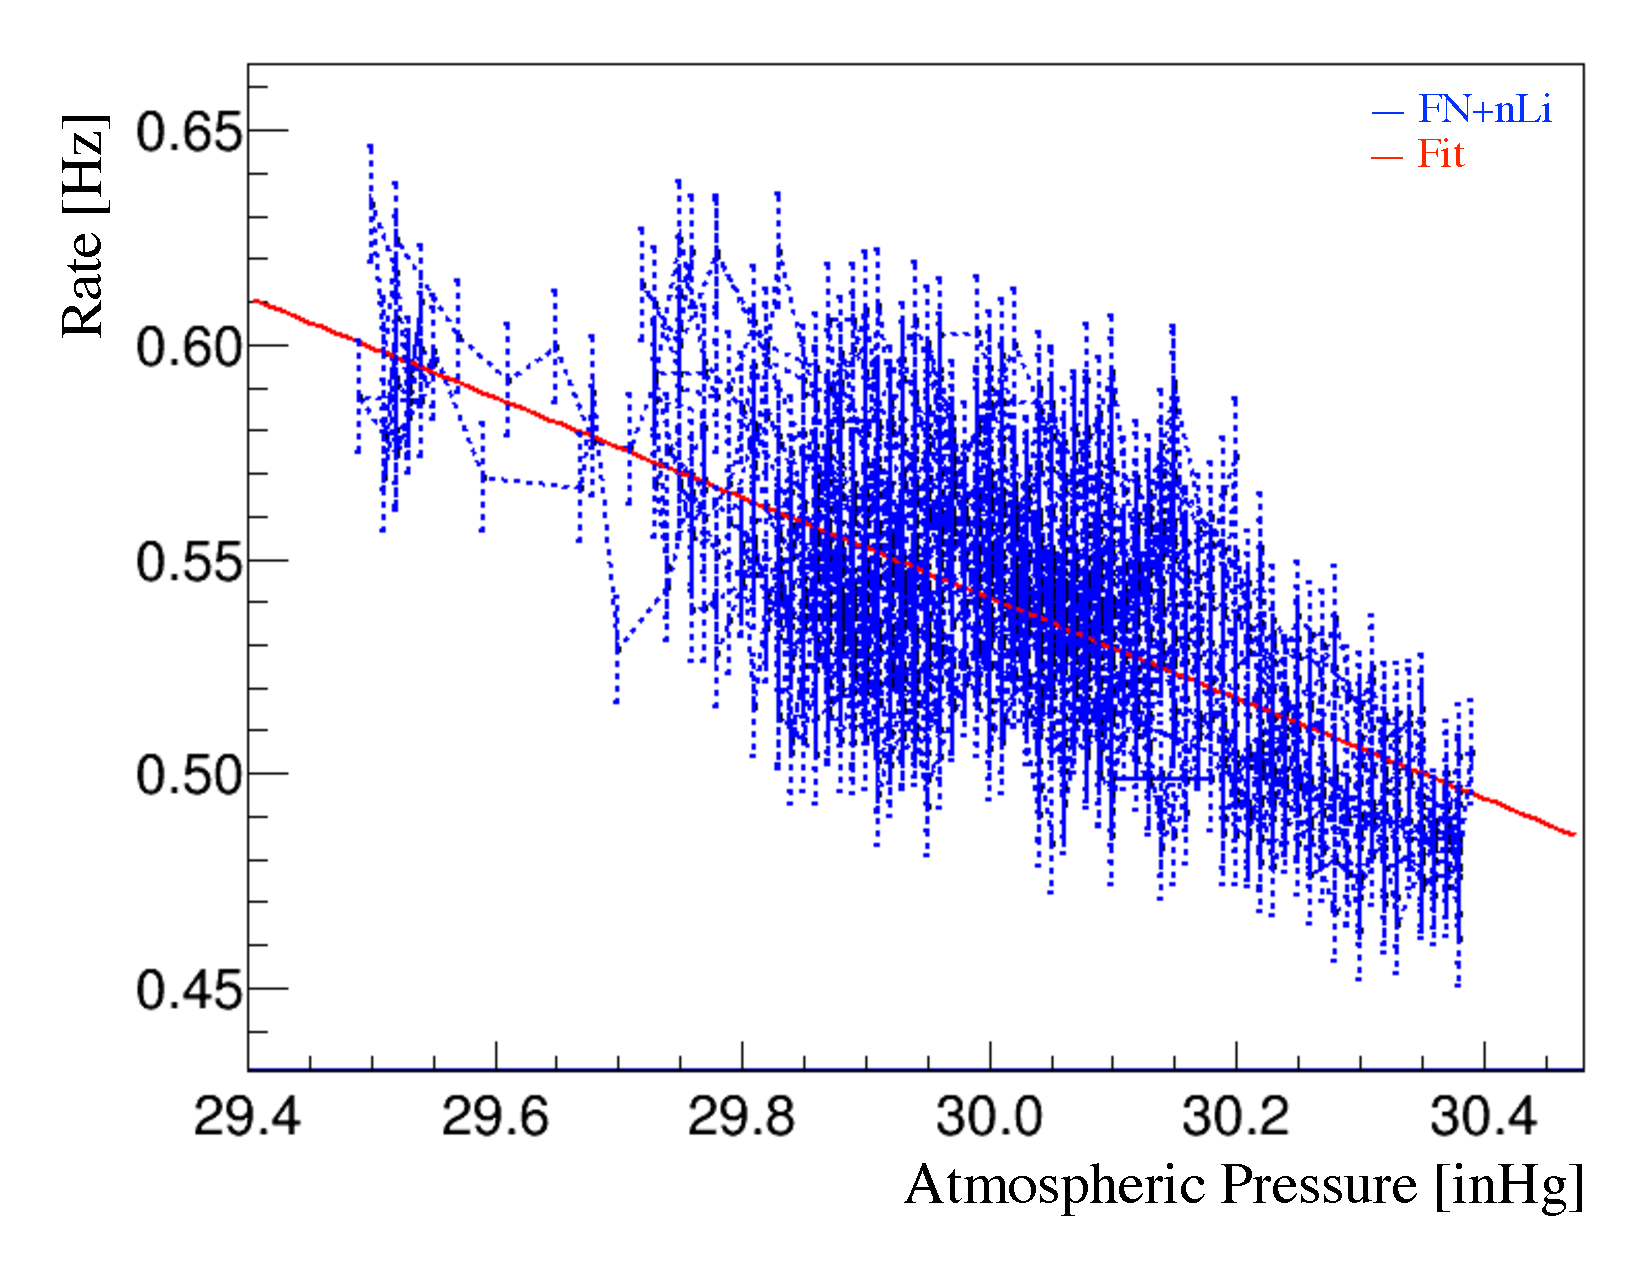
\includegraphics[width=0.95\linewidth]{tex/7-oscillation-images/FNnLi_RateVsPressure}
		%\caption{}
		\label{fig:fnnliratevspressure}
	\end{subfigure}
	\caption[]{(Left) The rate of fast neutron and nLi capture coincidences (blue) and pressure (red) versus time. (Right) FN+nLi rates as a function of pressure with a linear fit. \cite{Kyzylova2370:2018}}
	\label{fig:atm}
\end{figure}


Figure~\ref{fig:atm} shows the rate of these coincident events and pressure versus time, along with rate versus pressure.
It can be seen that the event rate and pressure are inversely correlated. 
The rate of FN+nLi events as a function of pressure was fit with a linear function and the results of the fit were used to define the atmospheric correction, $k_p$, according to
\begin{equation}
k_p = \frac{m \cdot \bar{p}_{on} + c}{m \cdot \bar{p}_{off} + c}
\end{equation}
where $m$ and $c$ are the slope and y-intercept of the fit and $\bar{p}_{on (off)}$ is the average pressure during reactor on (off).
For this analysis the atmospheric correction was found to be $<$ 1\%.


\subsection{Background Subtraction}

To obtain the final measured IBD events the correlated and accidental events are subtracted for both reactor on and off time periods.
Due to differences in reactor on and off exposure time, as well as differences between accidental and coincidental acceptance time windows, accidental and reactor off events have to be correctly scaled.
Therefore, the number of IBD candidates, $N_{IBD}$, is measured as:
\begin{equation}
\begin{split}
	N_{IBD} &= N_{corr-acc, on} - k_p \cdot N_{corr-acc, off} \\
				 &= N_{corr, on} - \frac{\Delta t_{corr}}{\Delta t_{acc}} N_{acc, on} - k_p \frac{t_{on}}{t_{off}}\left(N_{corr, off} - \frac{\Delta t_{corr}}{\Delta t_{acc}}N_{acc,off}\right)
\end{split}
\end{equation}


\section{Data Set}

The dataset used in this analysis consists of 30.26 (33) reactor on and 26.19 (28) reactor off effective (calendar) days.
The rate of correlated and accidental rates for each of these periods are listed in Table~\ref{tab:datastats}.
A total of 25461 IBD events were detected (771/day), with a signal-to-background ratio of 2.20 and 1.32 for accidental and correlated background, respectively.
The correlated and accidental rates per day as a function of time for events in the prompt energy region (0.8, 7.2) MeV can be seen in Figure~\ref{fig:evtrates}.

Due to current instabilities observed in some PMT's during the data-taking period 31 segments were excluded in this analysis: (0, 1, 2, 3, 4, 5, 6, 9, 10, 11, 12, 13, 18, 21, 23, 24, 27, 32, 34, 40, 44, 52, 68, 79, 86, 102, 115, 122, 127, 130, 139).
Two segments not in the outer shell were also added to the non-fiducial volume due to high background rates: (25, 26).
These two segments exist in a corner of the detector that does not sit on the monolith and therefore they see many $\gamma$-rays from beam lines under the floor.

\begin{table}[H]
\begin{tabular}{|c|c|c|c|}
	\hline 
	\textbf{Reactor} & \textbf{Event Type} & \textbf{Time [days]} & \textbf{Counts} \\ 
	\hline 
	& Correlated + Accidental &  & 56378 $\pm$ 1708 \\ 
	On & Accidental (scaled) & 30.26 & 11580 $\pm$ 12 \\ 
	& Correlated &  & 44797 $\pm$ 238 \\ 
	\hline 
	& Correlated + Accidental (scaled) & & 20262 $\pm$ 153   \\ 
	Off &  Accidental (scaled) & 26.19  & 925 $\pm$ 4   \\ 
	& Correlated (scaled) & & 19337 $\pm$ 153 \\ 
	\hline 
	\hline 
	& Signal &  & 25461 $\pm$ 238 (771/day) \\ 
	\hline 
\end{tabular} 
\caption{The total number of correlated and accidental events in the prompt energy region (0.8, 7.2) MeV for reactor on and off periods. Time refers to exposure time. The gap in data corresponds to a detector maintenance period.}
\label{tab:datastats}
\end{table}

\begin{figure}[H]
	\centering
	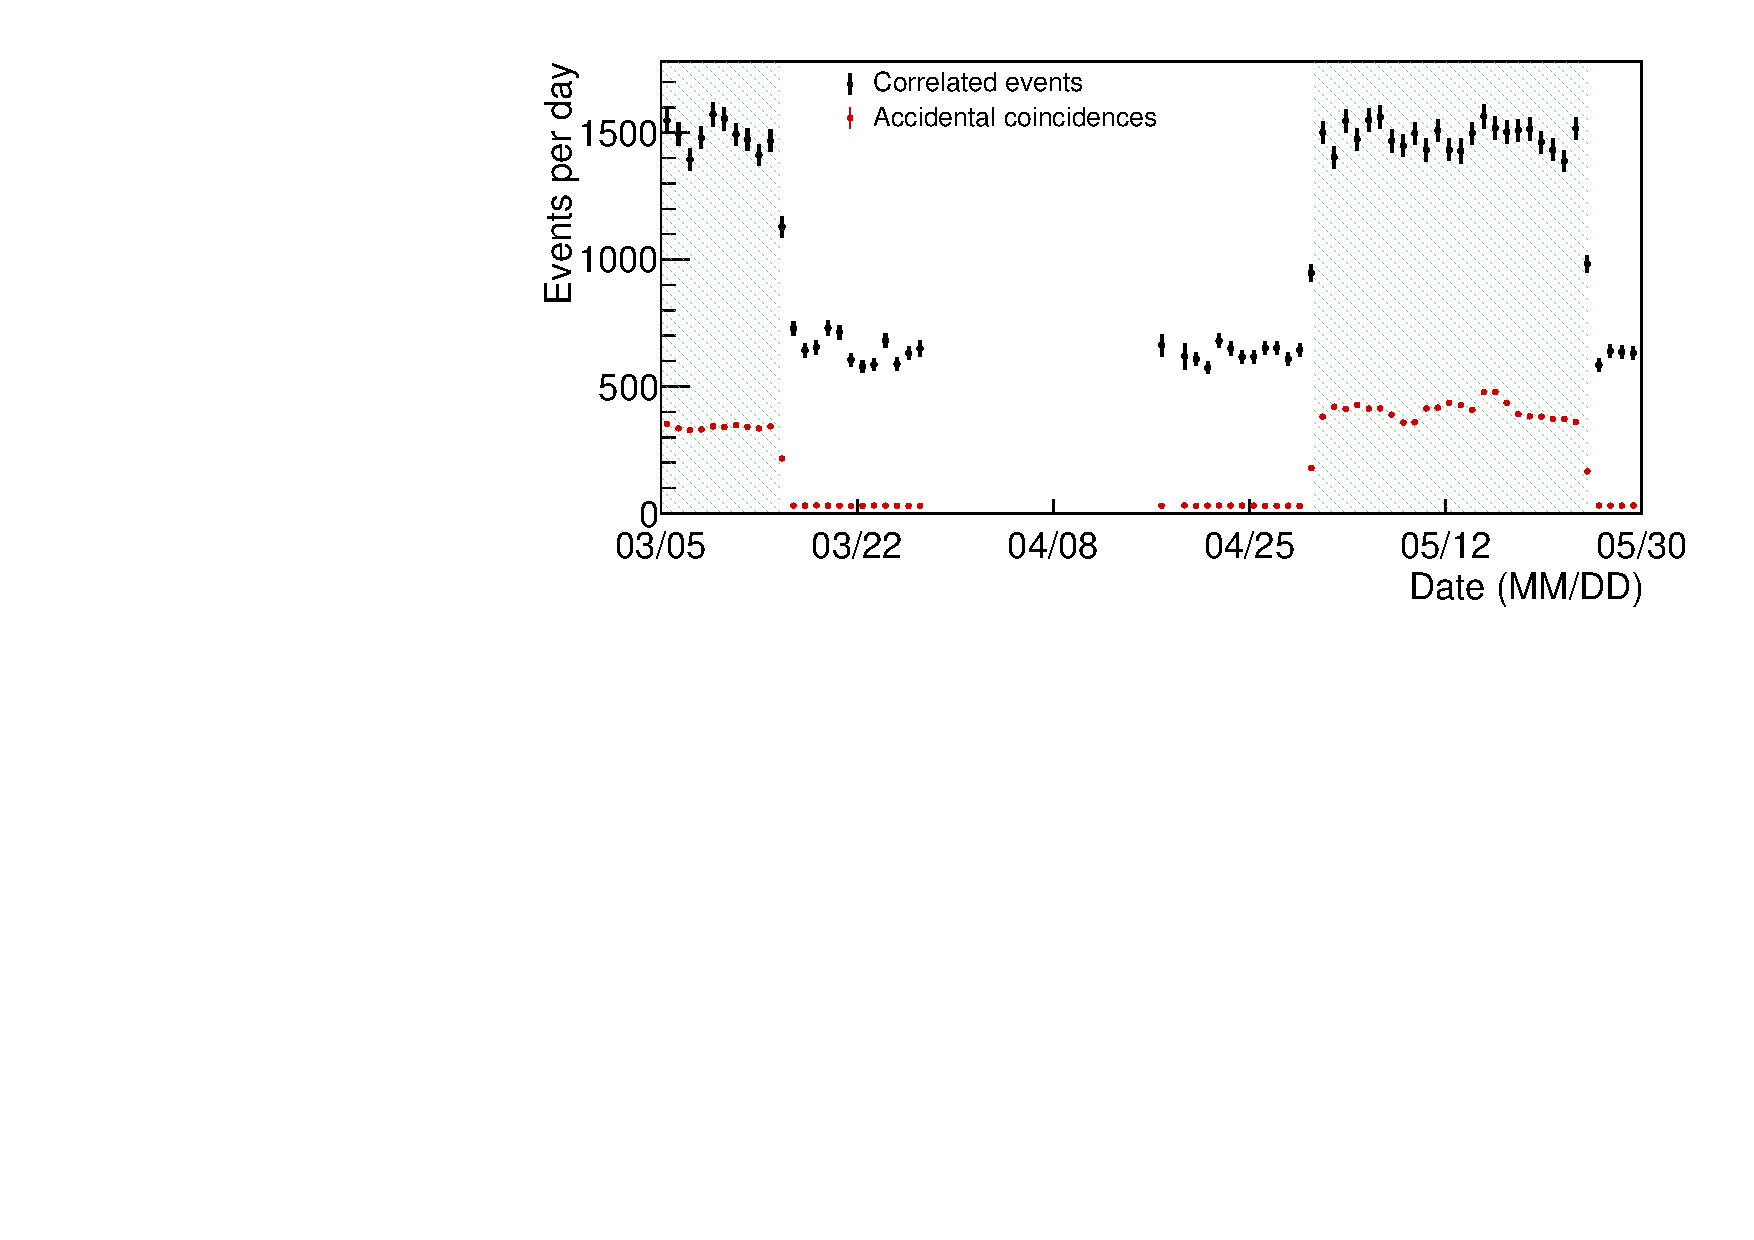
\includegraphics[width=0.7\linewidth]{tex/7-oscillation-images/EvtRates}
	\caption{Accidentals-subtracted IBD candidate event rate per day (black) and measured accidental rate (red) as a function of time. IBD candidate rates are corrected for dead time and exposure time. The shaded regions (green) are reactor on periods. Errors are statistical.}
	\label{fig:evtrates}
\end{figure}


\section{IBD Rates versus Basline}


\begin{figure}[H]
	\centering
	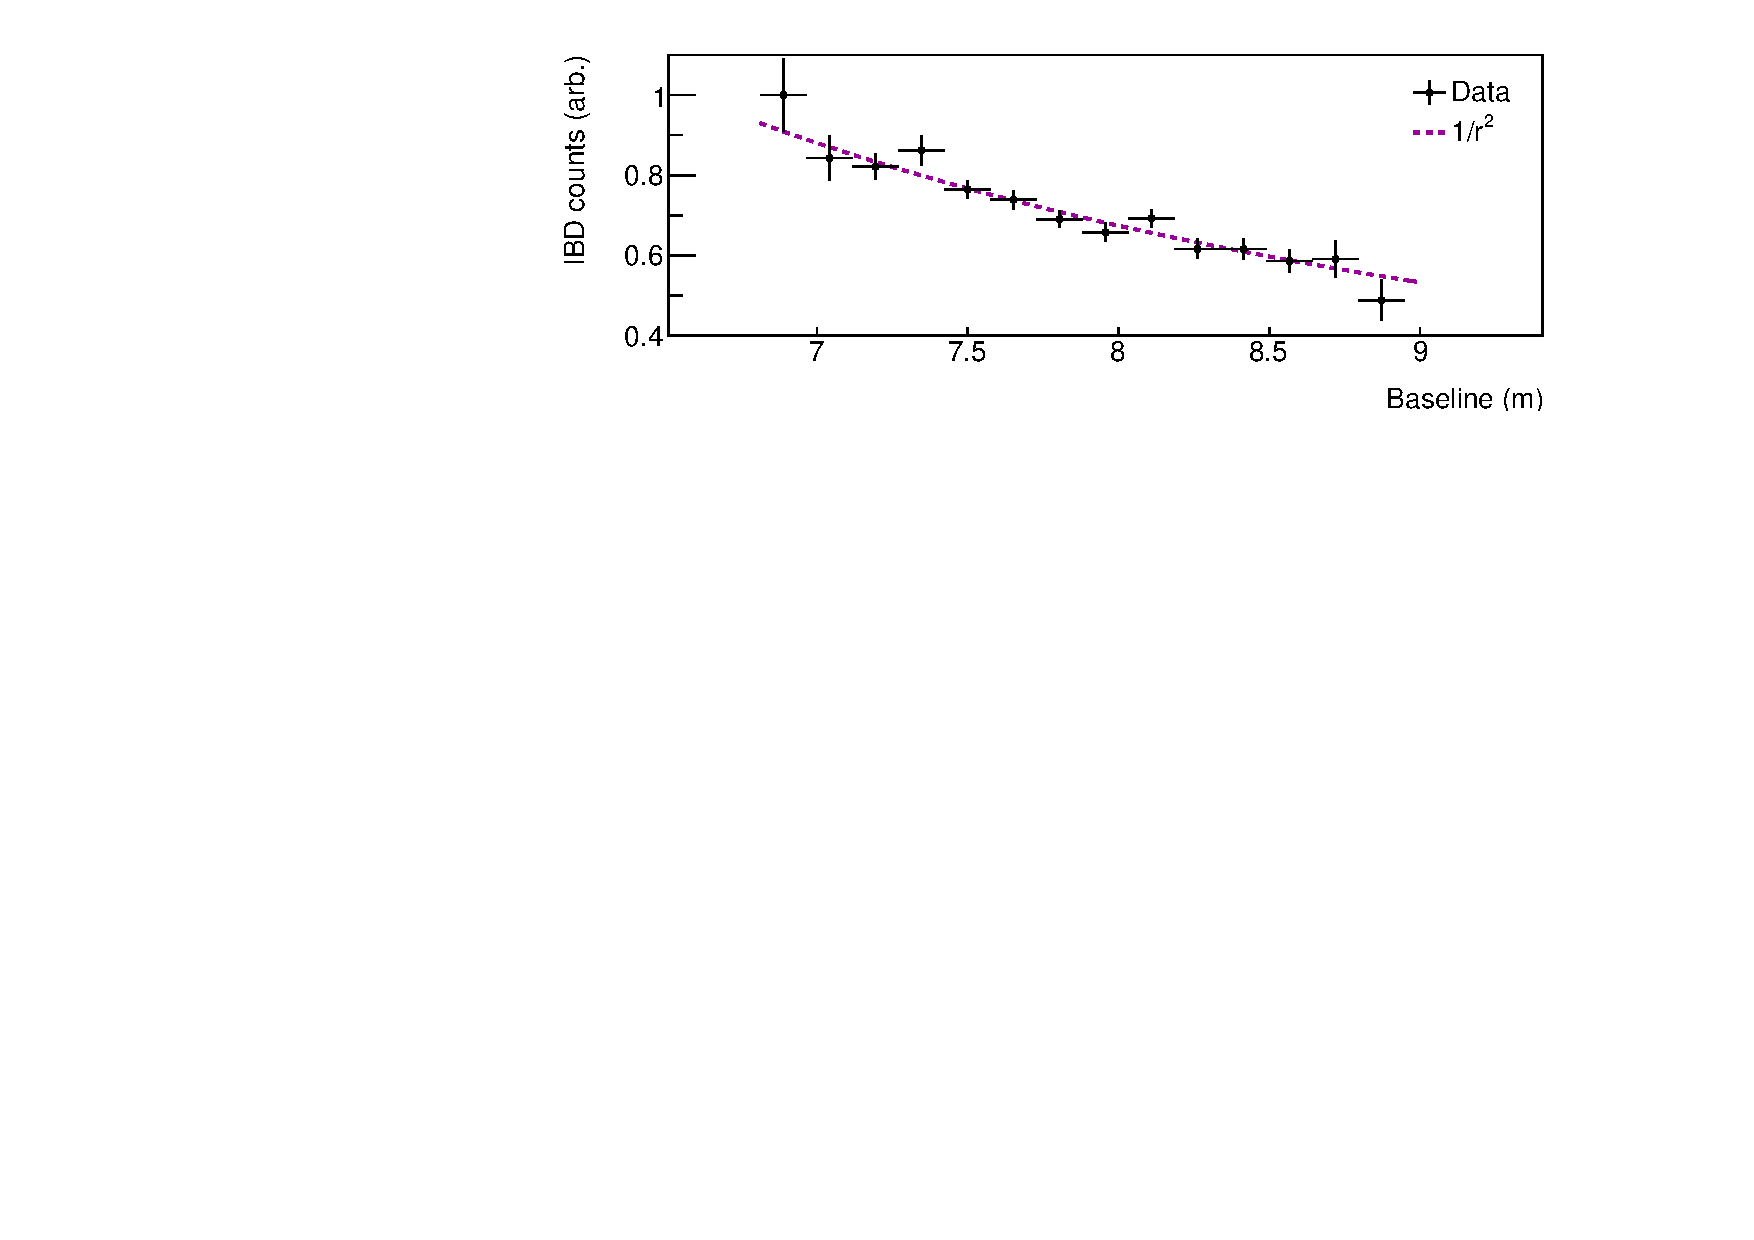
\includegraphics[width=1\linewidth]{tex/7-oscillation-images/IBDvsBaseline}
	\caption{}
	\label{fig:ibdvsbaseline}
\end{figure}



\section{Oscillation Search Result}

The construction of PROSPECT as a segmented detector allows the comparison of $\bar{\nu_e}$ spectrum between baselines rather than to a predicted reactor $\bar{\nu_e}$ spectrum. 
Therefore, the search for a sterile neutrino was carried out by comparing the measured IBD spectrum as a function of baseline (the L vs E spectrum) to a predicted L vs E spectrum constructed using MC simulations. For this analysis 6 position (baseline) bins and 16 energy bins were used.

To compare the spectra at different baselines a covariance-matrix based $\chi^2$ test-statistic was built according to:
\begin{equation}	
	\chi^2 = \Delta^TV^{-1}_{tot}\Delta
\end{equation}
where $V_{tot}$ is a covariance matrix constructed from the statistical and systematic uncertainties.
$\Delta$ is a 96-element vector representing the relative agreement between the measured ($M_{l,e}$) and predicted ($P_{l,e}$) L vs E spectra in the $l^{th}$ baseline bin and $e^{th}$ energy bin:
\begin{equation}
	\Delta_{l,e} = M_{l,e} - M_e\frac{P_{l,e}}{P_e}.
\end{equation}
$M_e$ and $P_e$ are the detector-wide spectrum rates in the $e^{th}$ energy bin and are defined as
\begin{equation}
	M_e = \sum_{l=1}^{6}M_{l,e}~\textrm{and}~P_e = \sum_{l=1}^{6}P_{l,e}.
\end{equation}




\begin{figure}[H]
	\centering
	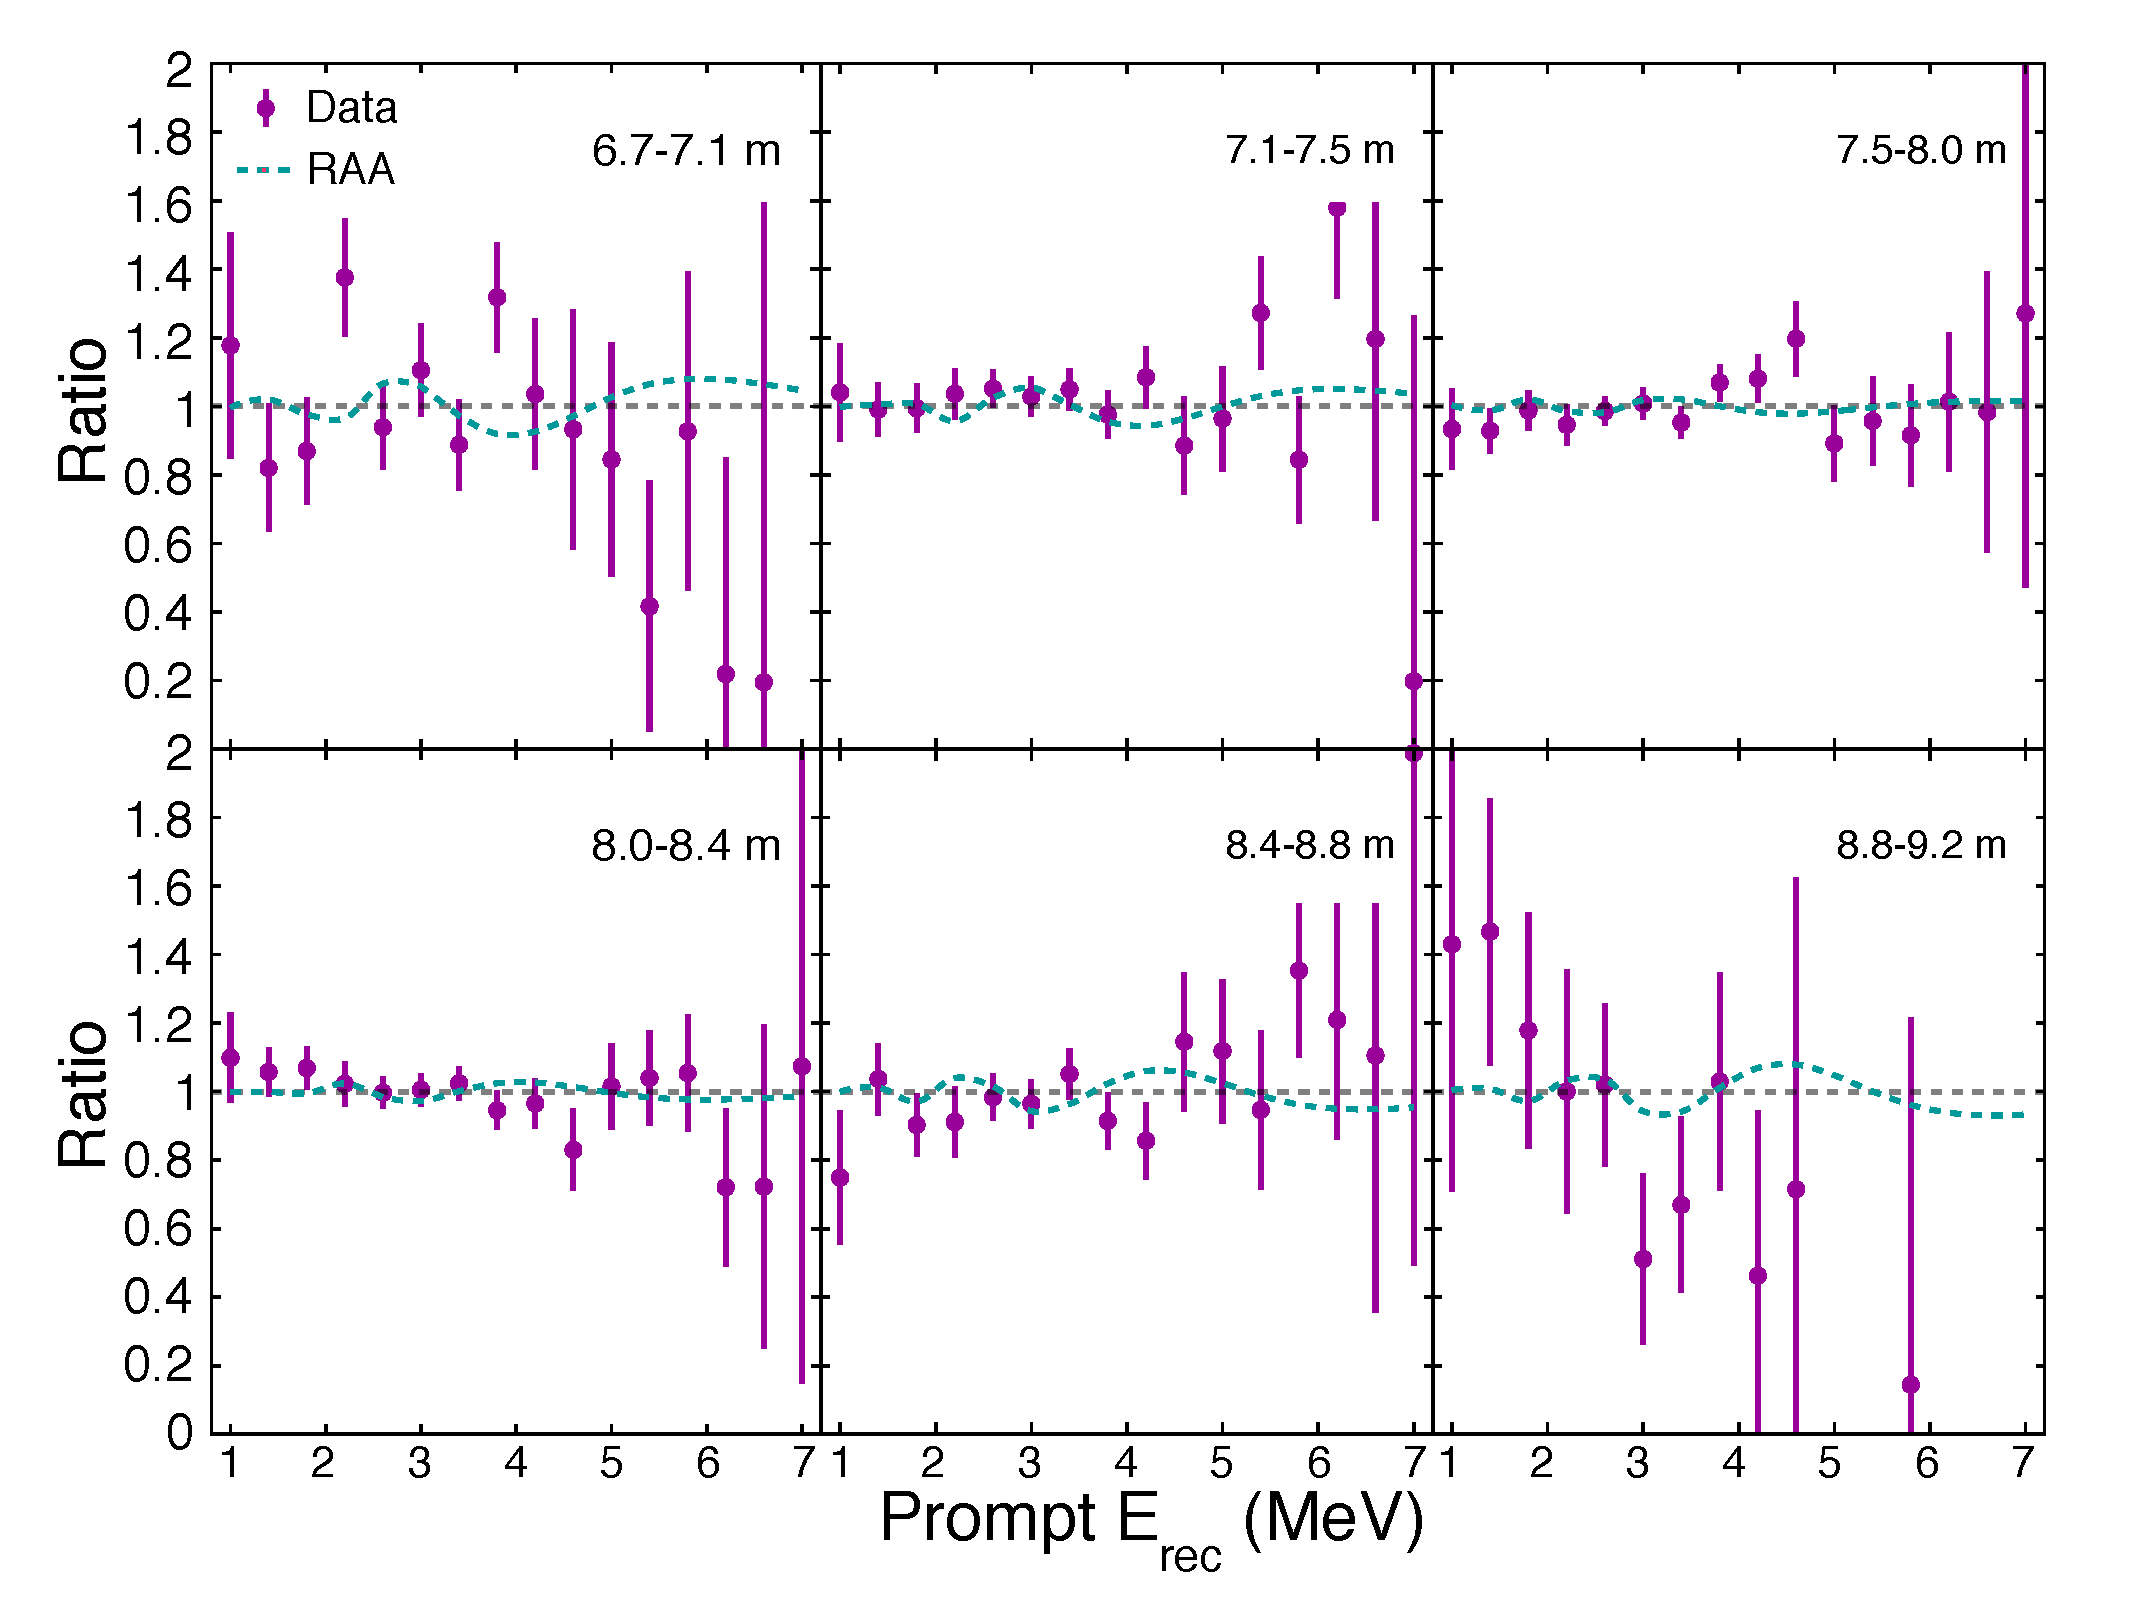
\includegraphics[width=0.7\linewidth]{tex/7-oscillation-images/BaselineSpectra}
	\caption{}
	\label{fig:baselinespectra}
\end{figure}

\begin{figure}[H]
	\centering
	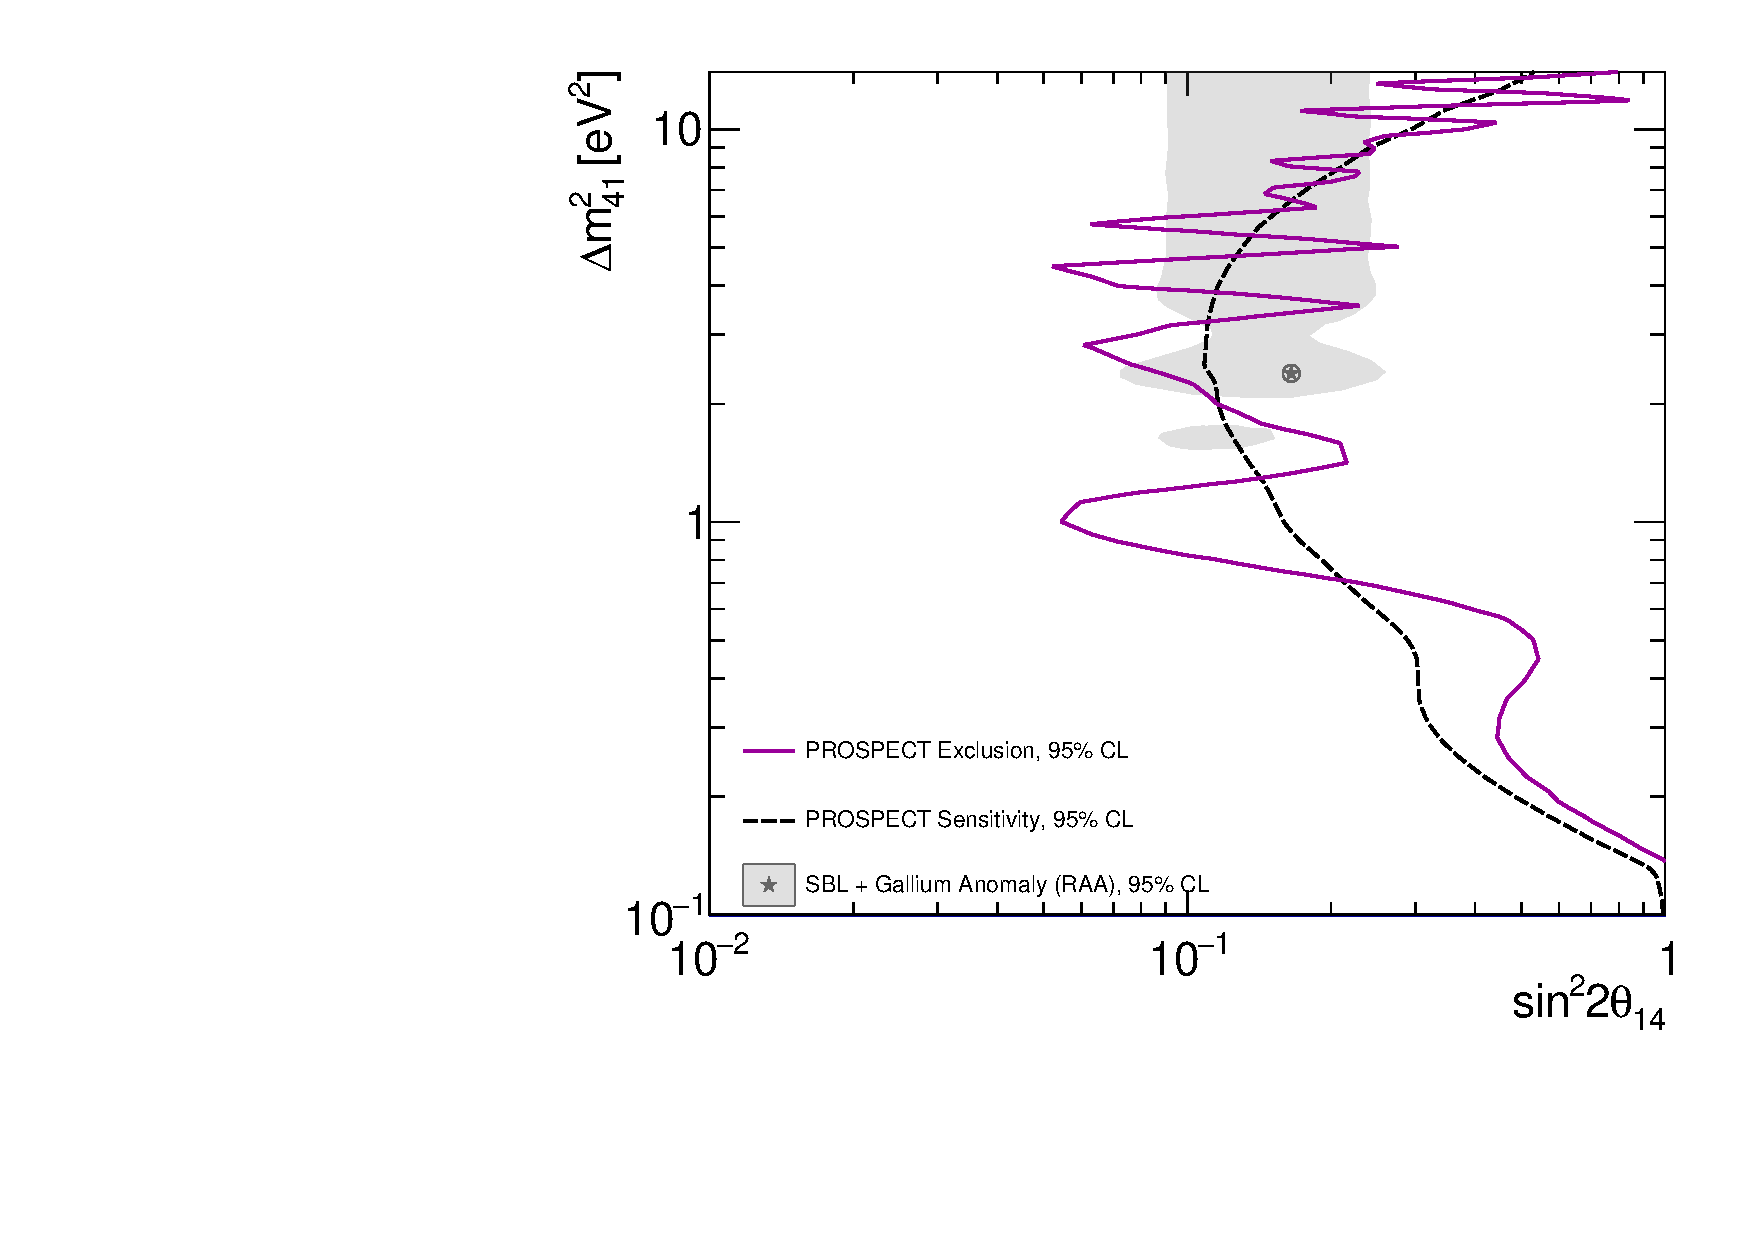
\includegraphics[width=0.7\linewidth]{tex/7-oscillation-images/Exclusion_Sensitivity_Final}
	\caption{}
	\label{fig:exclusionsensitivityfinal}
\end{figure}



\section{Measured Antineutrino Spectrum}
\begin{figure}[H]
	\centering
	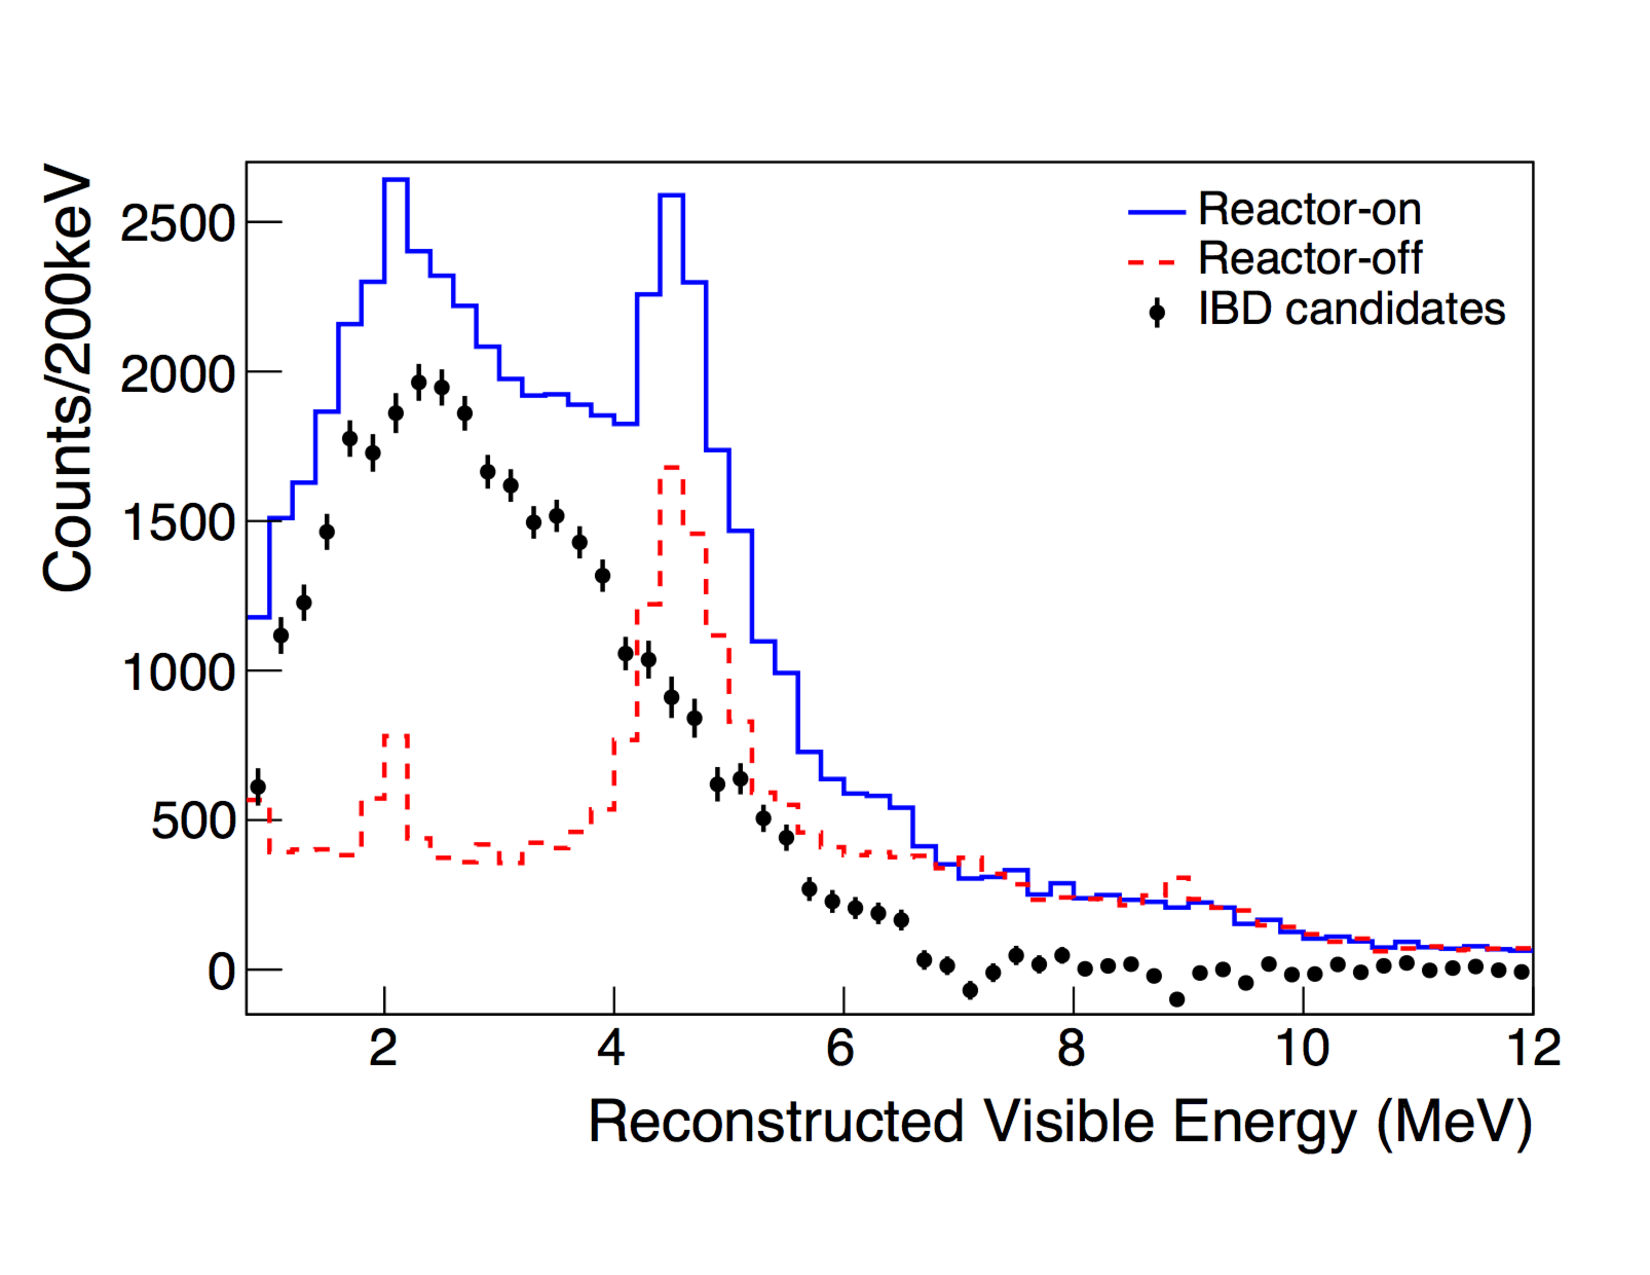
\includegraphics[width=0.7\linewidth]{tex/7-oscillation-images/Spectrum}
	\caption{}
	\label{fig:spectrumresults}
\end{figure}



